\documentclass{article}
\usepackage{fancyhdr}
\usepackage{amsthm}
\usepackage{etoolbox}
\usepackage{verbatim}
\usepackage{enumerate}
\usepackage{amsmath}
\usepackage{algorithmicx}
\usepackage{algorithm}
\usepackage{algpseudocode}
\usepackage{amssymb}
\usepackage{tikz}
	
\pagestyle{fancy}
\title{Chapter 27}
\author{Michelle Bodnar, Andrew Lohr}

\newcounter{curnum}
\setcounter{curnum}{0}

\newtheorem{th1}{Exercise} 
\newcommand{\calH}{\mathcal{H}}
\newcommand{\calX}{\mathcal{X}}
\newcommand{\calA}{\mathcal{A}}
\newcommand{\calY}{\mathcal{Y}}



\algblock{ParFor}{EndParFor}
% customising the new block
\algnewcommand\algorithmicparfor{\textbf{parallel for}}
\algnewcommand\algorithmicpardo{\textbf{do}}
\algnewcommand\algorithmicendparfor{\textbf{end}}
\algrenewtext{ParFor}[1]{\algorithmicparfor\ #1\ \algorithmicpardo}
\algrenewtext{EndParFor}{\algorithmicendparfor}

\begin{document}
\maketitle
\noindent\textbf{Exercise 27.1-1}\\

This modification is not going to affect the asymptotic values of the span work or parallelism. All it will do is add an amount of overhead that wasn't there before. This is because as soon as the $FIB(n-2)$ is spawned the spawning thread just sits there and waits, it does not accomplish any work while it is waiting. It will be done waiting at the same time as it would of been before because the $FIB(n-2)$ call will take less time, so it will still be limited by the amount of time that the $FIN(n-1)$ call takes.\\

\noindent\textbf{Exercise 27.1-2}\\

The computation dag is given in the image below.  The blue numbers by each strand indicate the time step in which it is executed. The work is 29, span is 10, and parallelism is 2.9.  \\

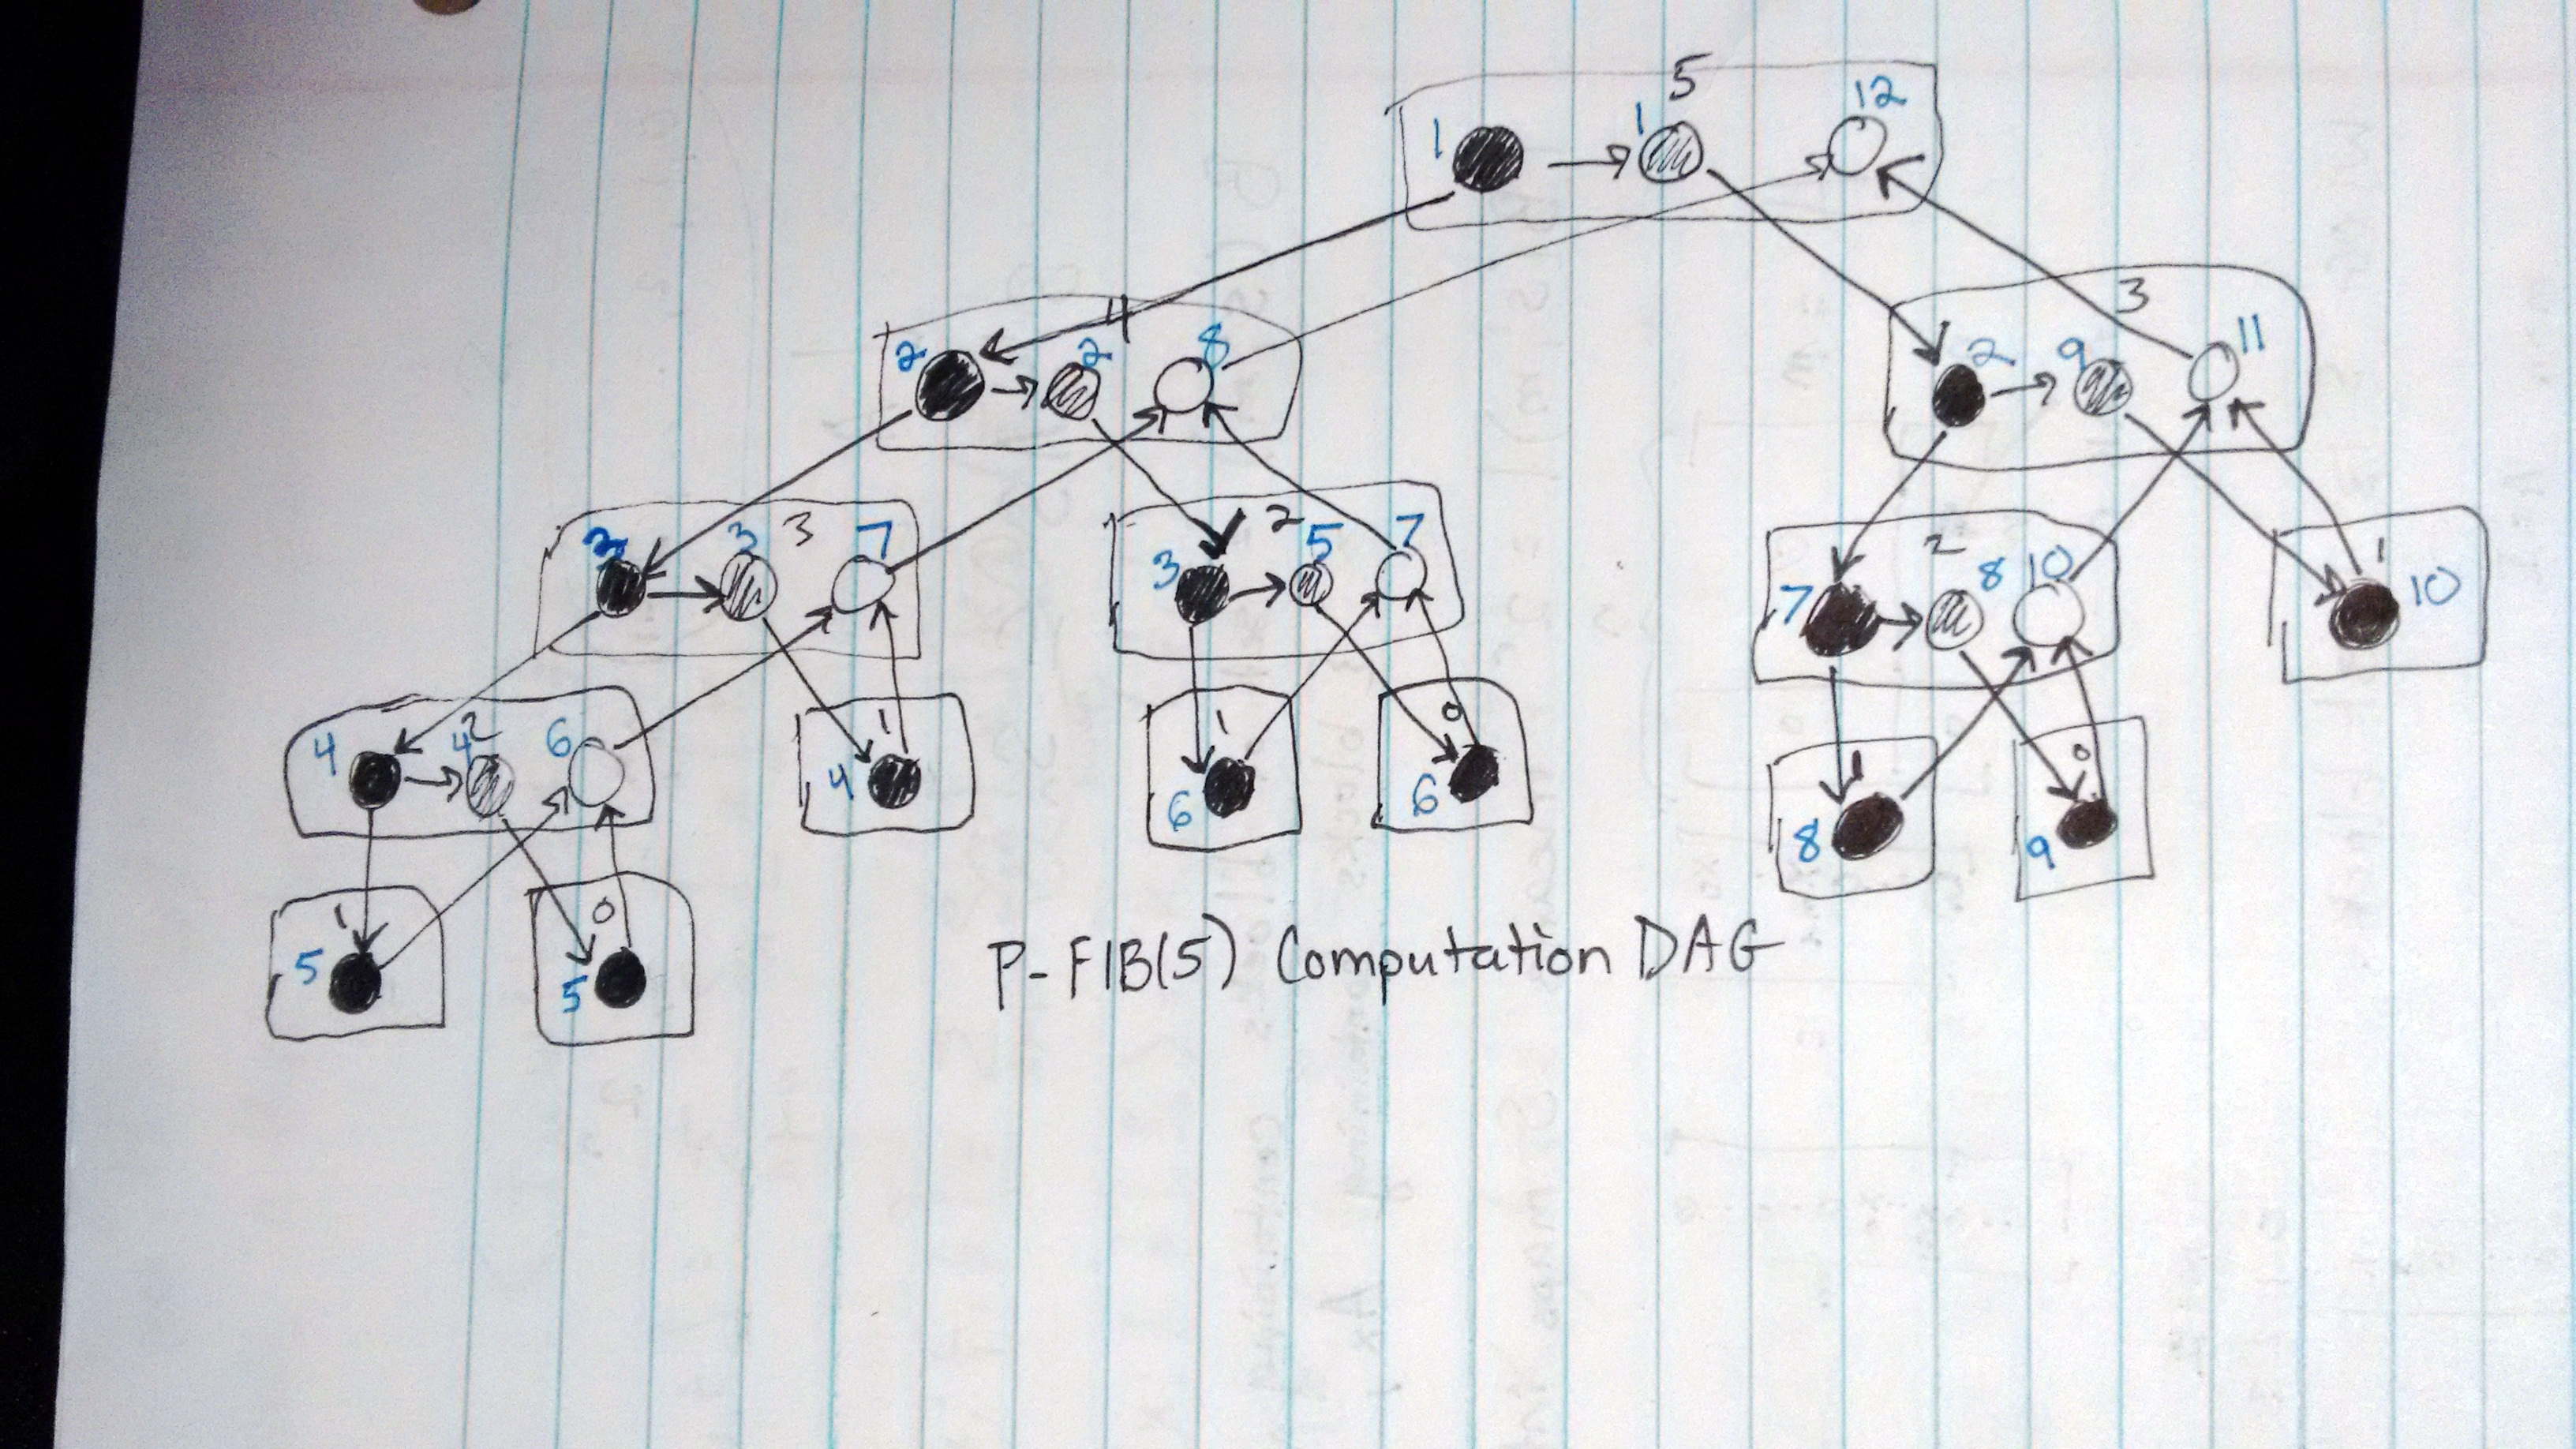
\includegraphics[scale=.1]{FibCompDag.jpg}\\

\noindent\textbf{Exercise 27.1-3}\\

Suppose that there are $x$ incomplete steps in a run of the program. Since each of these steps causes at least one unit of work to be done, we have that there is at most $(T_1-x)$ units of work done in the complete steps. Then, we suppose by contradiction that the number of complete steps is strictly greater than $\lfloor (T_1-x)/P\rfloor$. Then, we have that the total amount of work done during the complete steps is $P\cdot (\lfloor (T_1-x)/P\rfloor + 1) = P\lfloor (T_1-x)/P\rfloor +P =  (T_1-x) - ((T_1-x)\mod P) + P > T_1-x$. This is a contradiction because there are only $(T_1-x)$ units of work done during complete steps, which is less than the amount we would be doing. Notice that since $T_\infty$ is abound on the total number of both kinds of steps, it is a bound on the number of incomplete steps, x , so, 
\[
T_P \le \lfloor (T_1-x)/P\rfloor +x \le \lfloor (T_1-T_{\infty})/P\rfloor +T_{\infty} 
\]
Where the second inequality comes by noting that the middle expression, as a function of $x$ is monotonically increasing, and so is bounded by the largest value of $x$ that is possible, namely $T_{\infty}$.\\

\noindent\textbf{Exercise 27.1-4}\\

The computation is given in the image below.  Let vertex $u$ have degree $k$, and assume that there are $m$ vertices in each vertical chain.  Assume that this is executed on $k$ processors.  In one execution, each strand from among the $k$ on the left is executed concurrently, and then the $m$ strands on the right are executed one at a time.  If each strand takes unit time to execute, then the total computation takes $2m$ time.  On the other hand, suppose that on each time step of the computation, $k-1$ strands from the left (descendents of $u$) are executed, and one from the right (a descendent of $v$), is executed.  If each strand take unit time to executed, the total computation takes $m + m/k$.  Thus, the ratio of times is $2m/(m + m/k) = 2/(1+1/k)$.  As $k$ gets large, this approaches 2 as desired.  \\

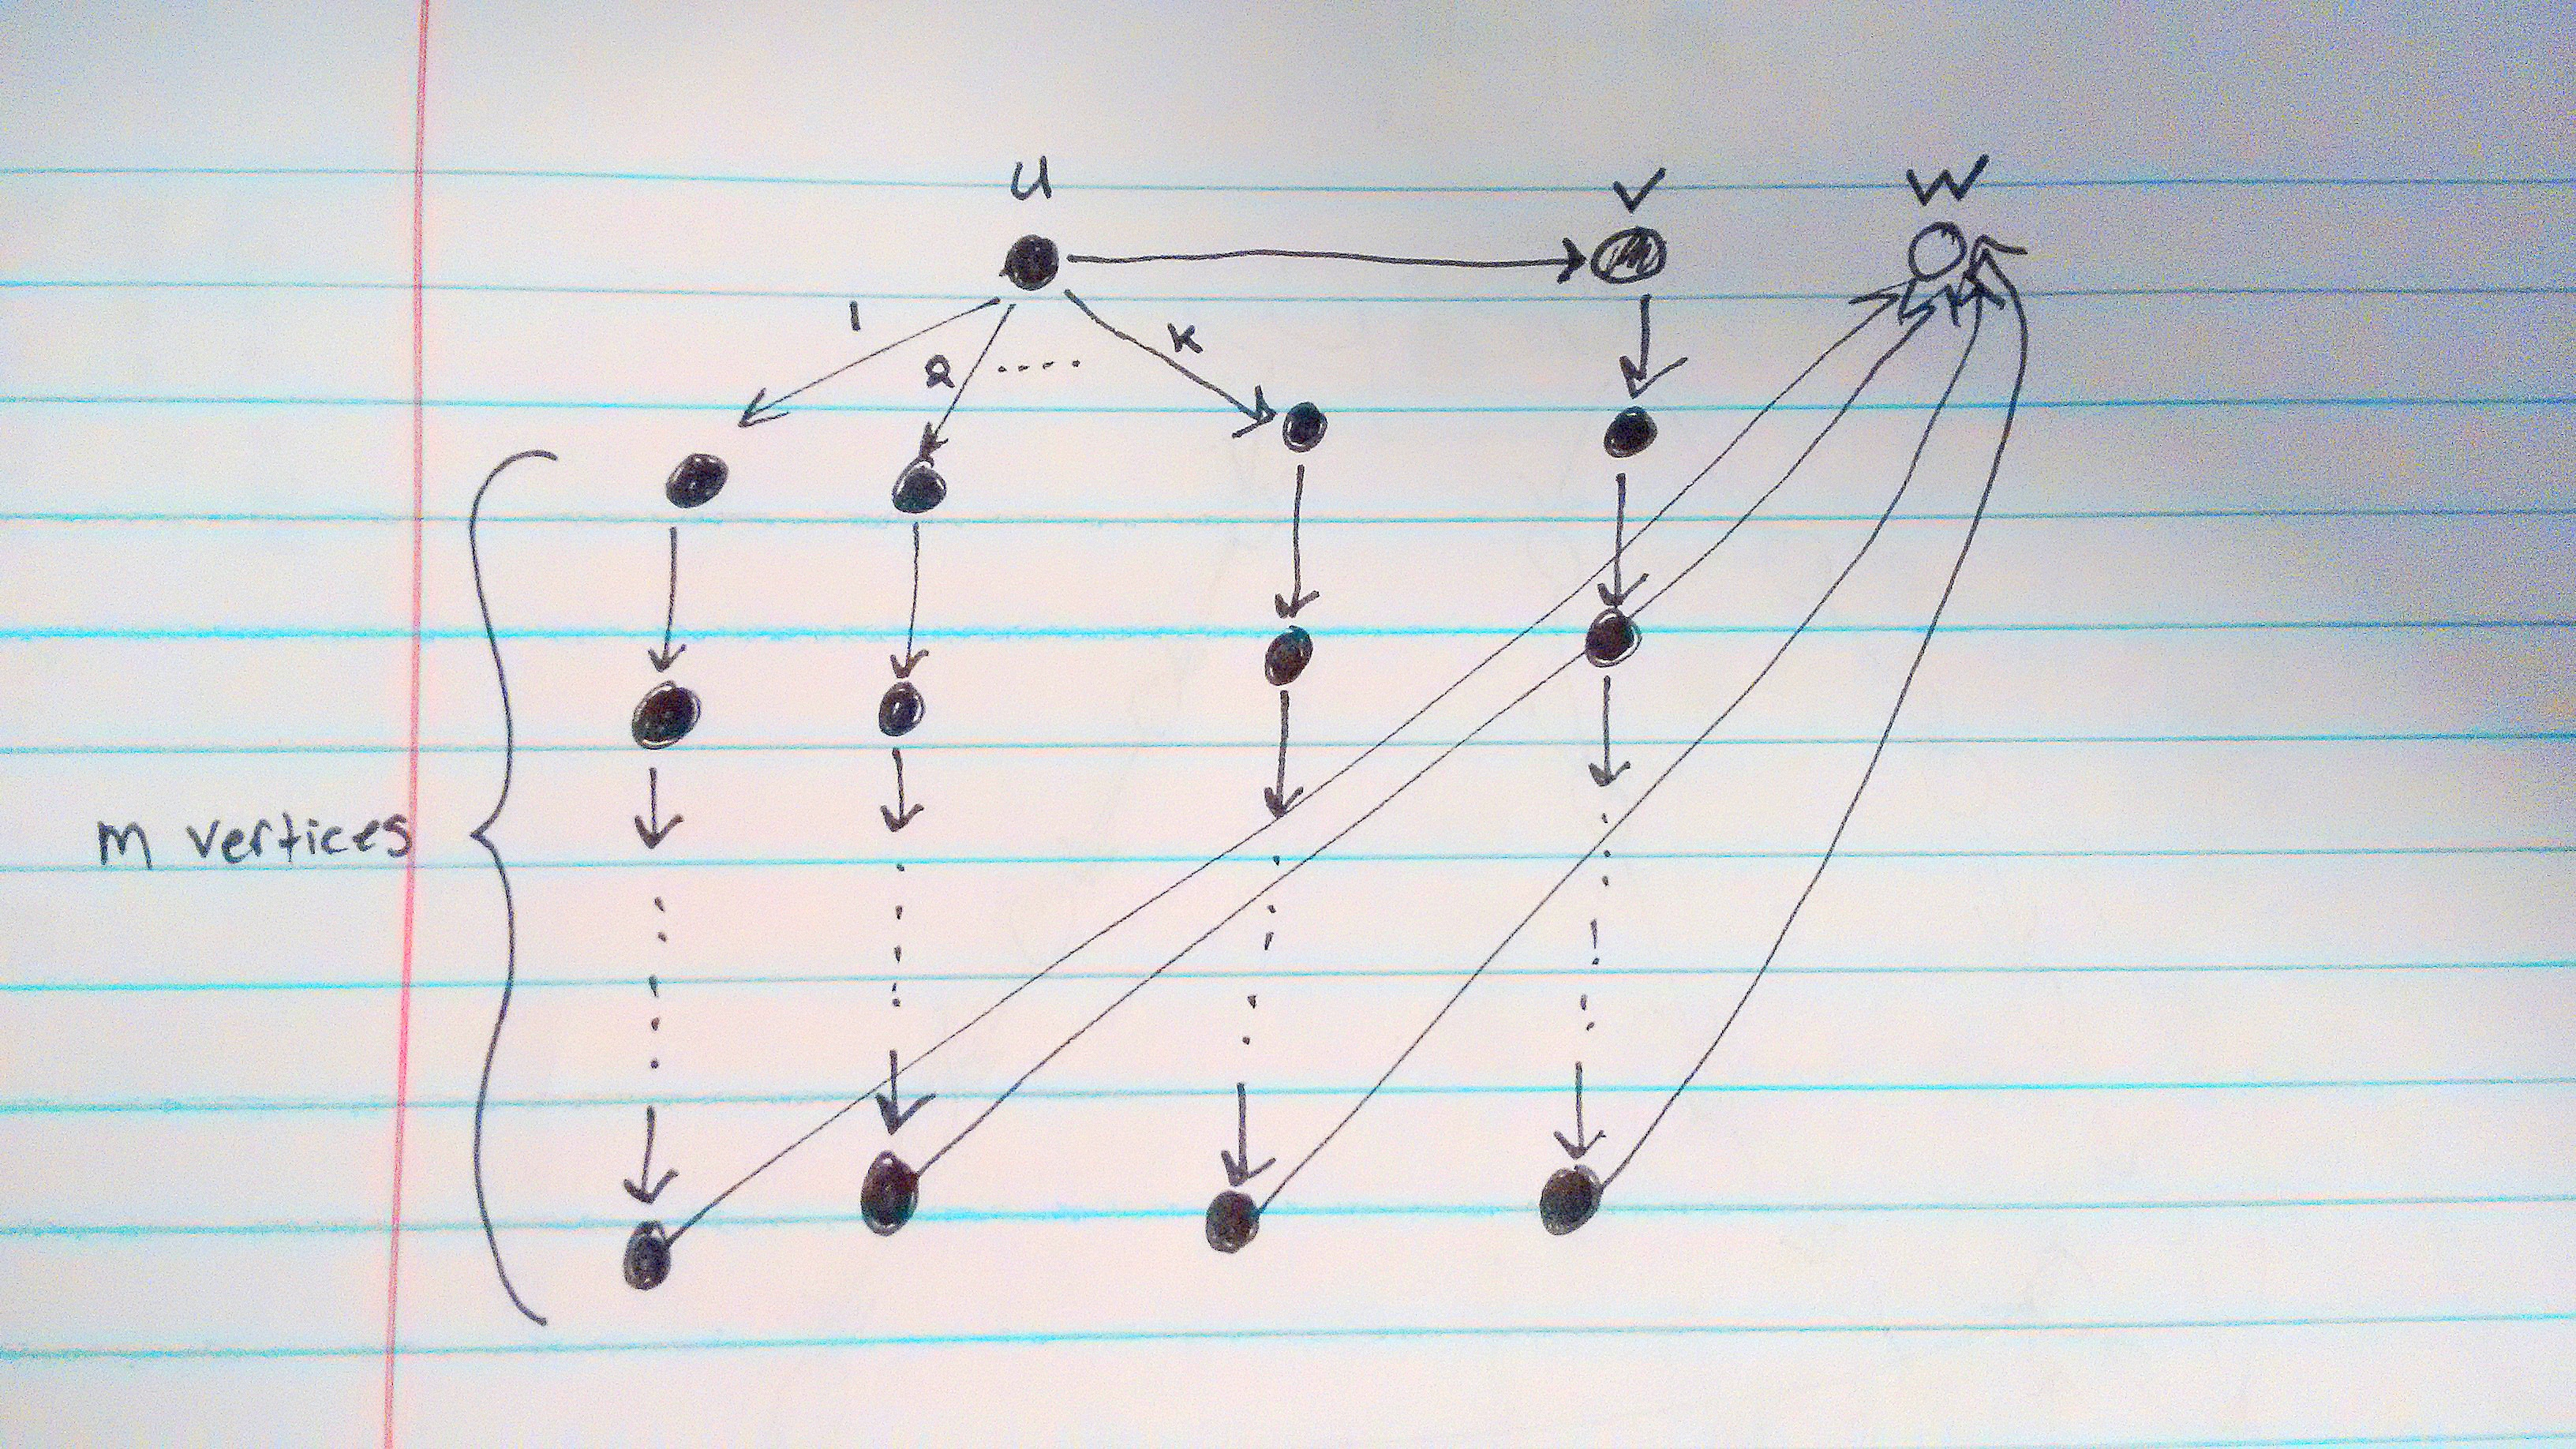
\includegraphics[scale=.1]{2CompDag.jpg}\\

\noindent\textbf{Exercise 27.1-5}\\

The information from $T_{10}$ applied to equation (27.5) give us that
\begin{align*}
42 &\le {T_1 - T_\infty}{10} + T_\infty
\end{align*}

which tell us that 
\begin{align*}
420 &\le T_1 +9 T_\infty
\end{align*}


Subtracting these two equations, we have that $100 \le 8 T_\infty$.

If we apply the span law to $T_64$, we have that $10\ge T_\infty$. Applying the work law to our measurement for $T_4$ gets us that $320 \ge  T_1$. Now, looking at the result of applying $(27.5)$ to the value of $T_10$, we get that
\[
420 \le T_1 + 9T_\infty \le 320 + 90 = 410
\]
a contradiction. So, one of the three numbers for runtimes must be wrong. However, computers are complicated things, and its difficult to pin down what can affect runtime in practice. It is a bit harsh to judge professor Karan too poorly for something that may of been outside her control (maybe there was just a garbage collection happening during one of the measurements, throwing it off).\\

\noindent\textbf{Exercise 27.1-6}\\

We'll parallelize the for loop of lines 6-7 in a way which won't incur races.  With the algorithm $P-PROD$ given below, it will be easy to rewrite the code.  For notation, let $a_i$ denote the $i^{th}$ row of the matrix $A$.

\begin{algorithm}
\caption{P-PROD(a,x,j,j')}
\begin{algorithmic}[1]
\If{$j== j'$}
\State \Return  $a[j] \cdot x[j]$
\EndIf
\State mid = $\left\lfloor \frac{j+j'}{2}\right\rfloor$
\State a' = spawn P-PROD(a,x,j,mid)
\State x' = P-PROD(a,x,mid+1,j')
\State sync
\State \Return a'+x'
\end{algorithmic}
\end{algorithm}

\begin{algorithm}
\caption{MAT-VEC(A,x)}
\begin{algorithmic}[1]
\State $n=A.rows$
\State let $y$ be a new vector of length $n$
\ParFor{$i=1$ to $n$}
	\State $y_i = 0$
\EndParFor
\ParFor{$i=1$ to $n$}
	\State $y_i = $ P-PROD$(a_i, x, 1, n)$
\EndParFor
\State \Return $y$
\end{algorithmic}
\end{algorithm}

\noindent\textbf{Exercise 27.1-7}\\

The work is unchanged from the serial programming case. Since it is flipping $\Theta(n^2)$ many entries, it does $\Theta(n^2)$ work. The span of it is $\Theta(\lg(n))$ this is because each of the parallel for loops can have its children spawned in time $\lg(n)$, so the total time to get all of the constant work tasks spawned is $2\lg(n) \in \Theta(\lg)$. Since the work of each task is $o(\lg(n))$, that doesn't affect the $T_\infty$ runtime. The parallelism is equal to the work over the span, so it is $\Theta(n^2/\lg(n))$.\\

\noindent\textbf{Exercise 27.1-8}\\

The work is $\Theta(1 + \sum_{j=2}^n j-1) = \Theta(n^2)$. The span is $\Theta(n)$ because in the worst case when $j=n$, the for-loop of line 3 will need to execute $n$ times.  The parallelism is $\Theta(n^2) / \Theta(n) = \Theta(n)$.\\

\noindent\textbf{Exercise 27.1-9}\\

We solve for P in the following equation obtained by setting $T_P = T_P'$.
\begin{align*}
\frac{T_1}{P}+T_\infty &= \frac{T_1'}{P} + T_\infty'\\
\frac{2048}{P} + 1 &= \frac{1024}{P}+8\\
\frac{1024}{P} &= 7\\
\frac{1024}{7} &=P
\end{align*}

So we get that there should be approximately 146 processors for them to have the same runtime.\\



\noindent\textbf{Exercise 27.2-1}\\

%diagrams -_-

\noindent\textbf{Exercise 27.2-2}\\

See the computation dag in the image below.  Assuming each strand takes unit time, the work is 26, the span is 16, and the parallelism is 1.625.\\

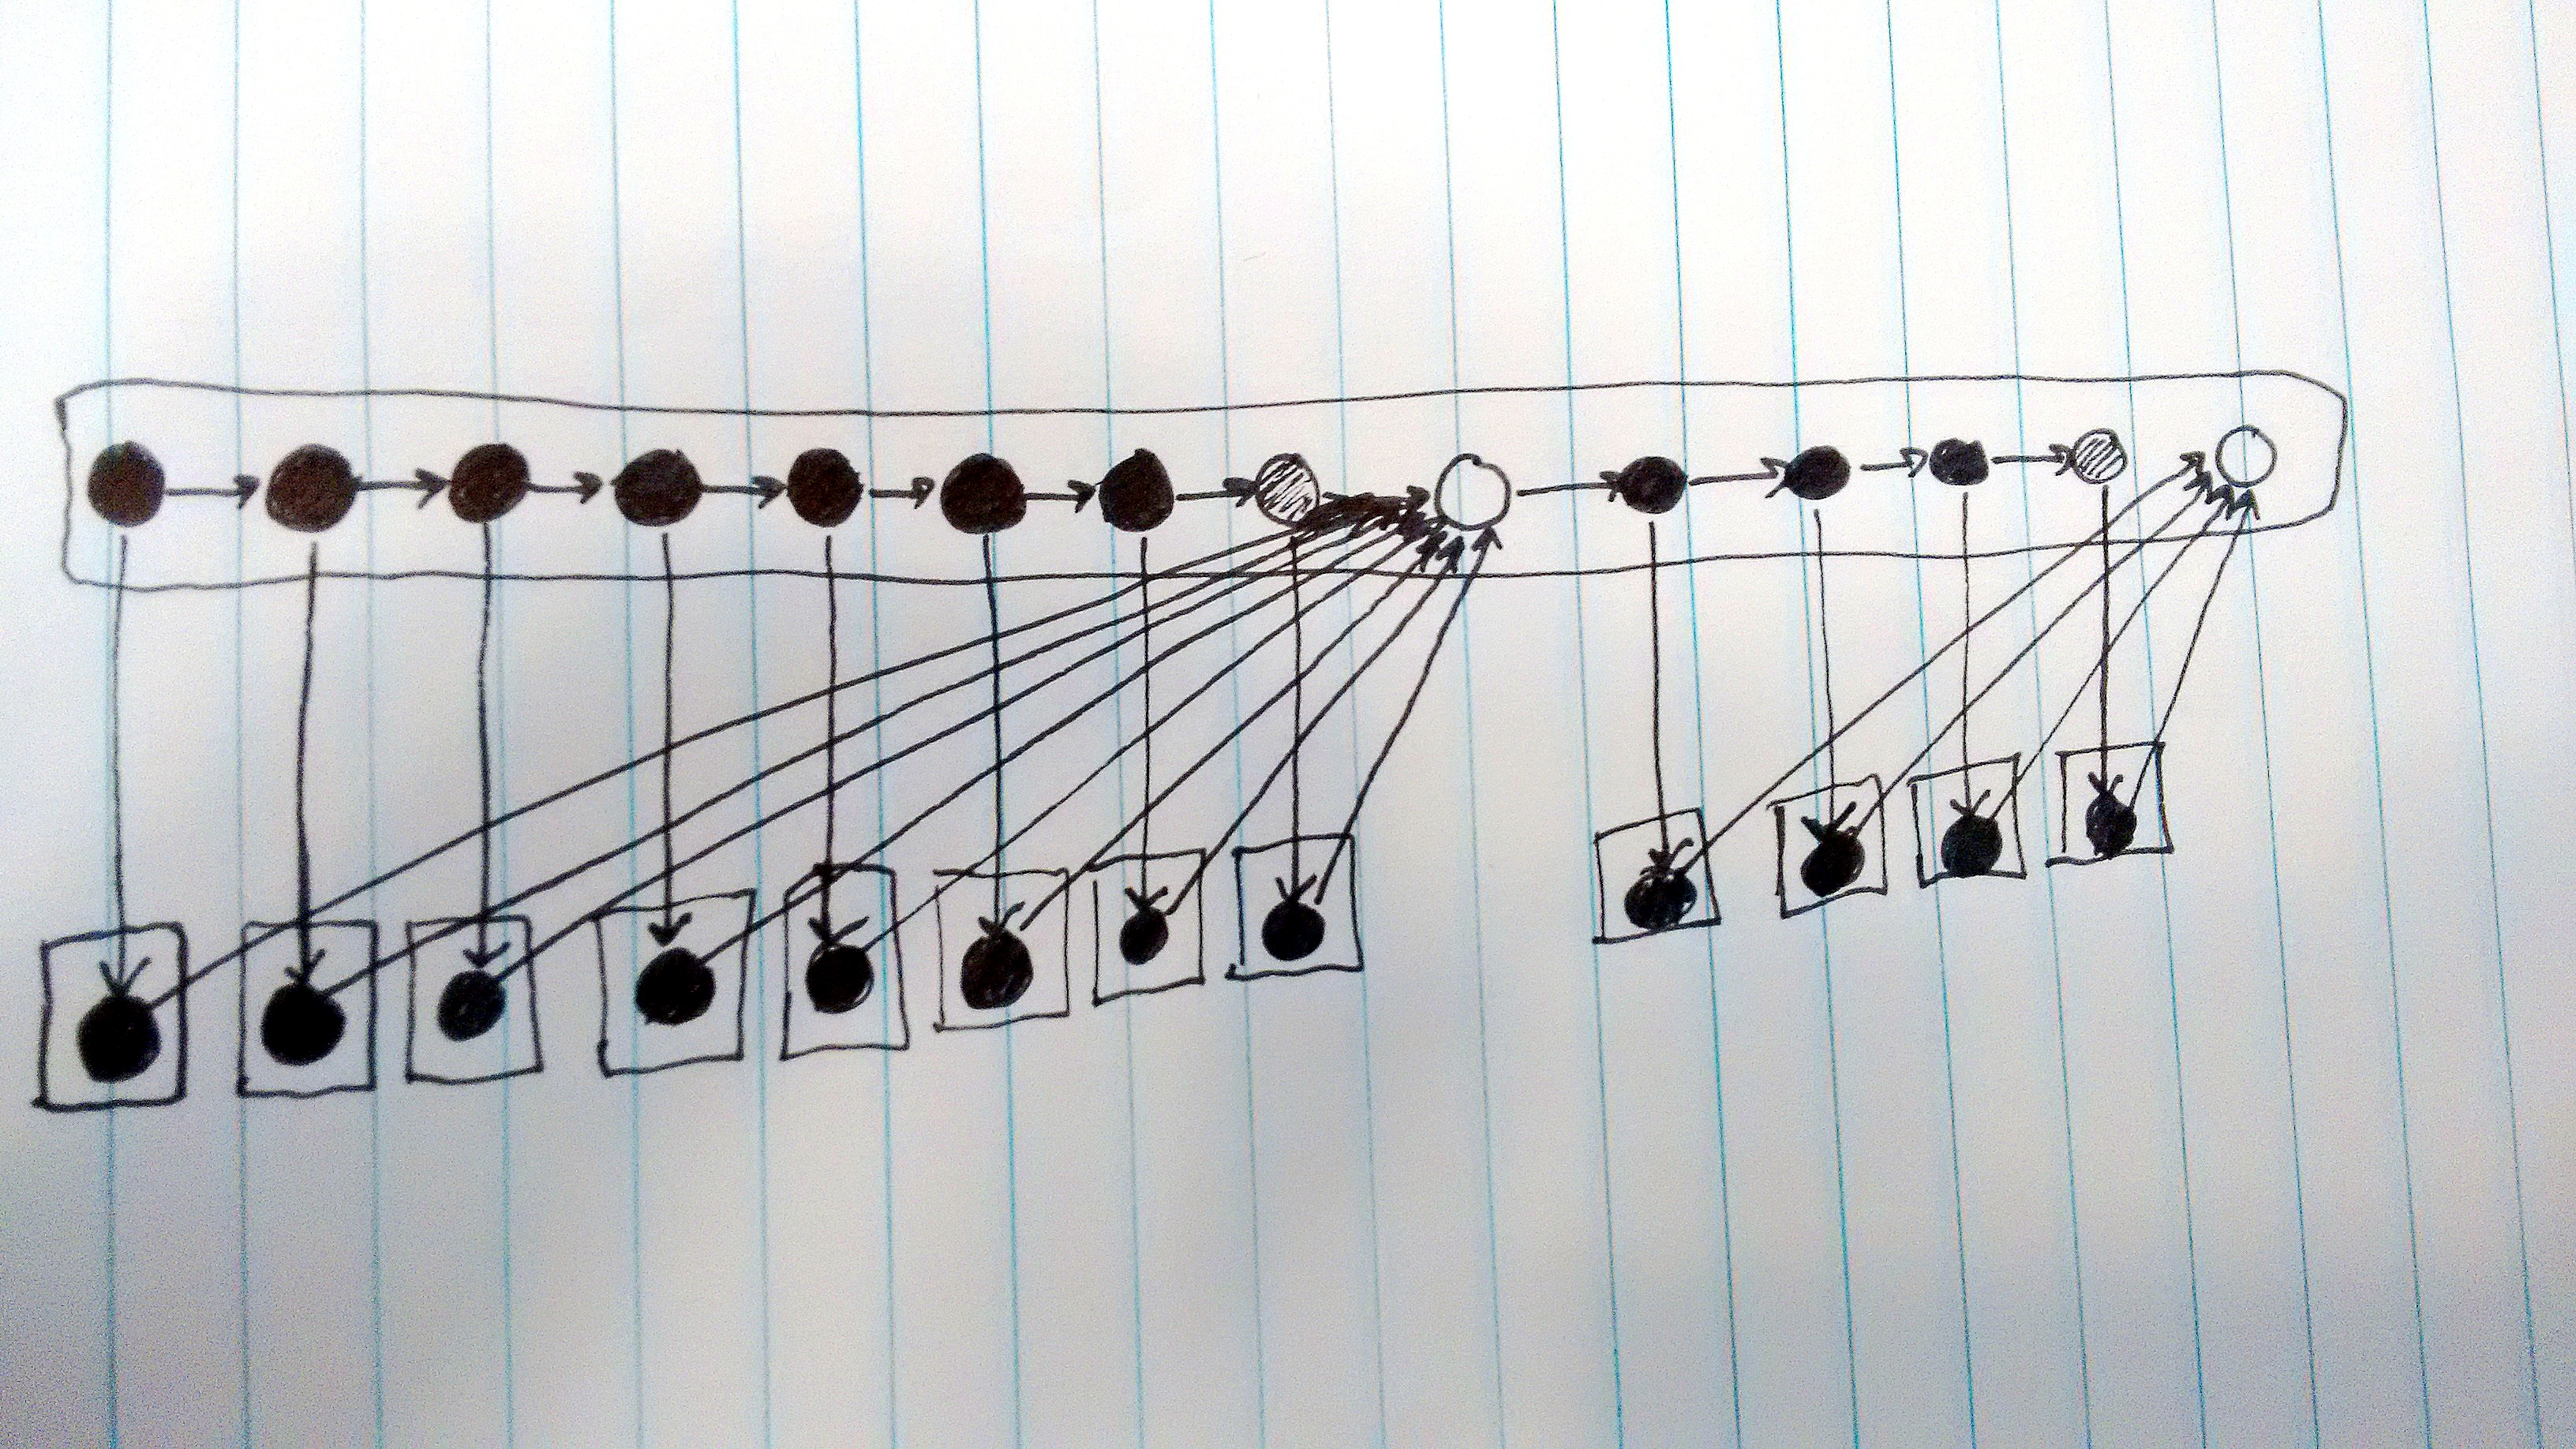
\includegraphics[scale=.1]{MatMulRecDag}\\

\noindent\textbf{Exercise 27.2-3}\\

We perform a modification of the P-SQUARE-MATRIX-MULTIPLY algorithm. Basiglly, as hinted in the text, we will parallelize the innermost for loop in such a way that there aren't any data races formed. To do this, we will just define a parallelized dot product procedure. This means that lines 5-7 can be replaced by a single call to this procedure. P-DOT-PRODUCT computes the dot dot product of the two lists between the two bounds on indices.

\begin{algorithm}
\caption{P-DOT-PROD(v,w,low,high)}
\begin{algorithmic}
\If{low == high}
\State \Return  v[low] = v[low]
\EndIf
\State mid = $\left\lfloor \frac{low+high}{2}\right\rfloor$
\State x = spawn P-DOT-PROD(v,w,low,mid)
\State y = P-DOT-PROD(v,w,mid+1,high)
\State sync
\State \Return x+y
\end{algorithmic}
\end{algorithm}

Using this, we can use this to modify P-SQUARE-MATRIX-MULTIPLY

\begin{algorithm}
\caption{MODIFIED-P-SQUARE-MATRIX-MULTIPLY}
\begin{algorithmic}
\State n = A.rows
\State let C be a new $n\times n$ matrix
\ParFor{i=1 to n}
\ParFor{j=1 to n}
\State $c_{i,j} =$ P-DOT-PROD$(A_{i,\cdot},B_{\cdot,j},1,n)$
\EndParFor
\EndParFor
\State \Return C
\end{algorithmic}
\end{algorithm}

Since the runtime of the inner loop is $O(\lg(n))$, which is the depth of the recursion. Since the paralel for loops also take $O(\lg(n))$ time. So, since the runtimes are additive here, the total span of this procedure is $\Theta(\lg(n))$. The total work is still just $O(n^3)$ Since all the spawnging and recursing couls be replaced with the normal serial version once there anren't enough free processors to handle all of the spawned calls to P-DOT-PRODUCT. \\

\noindent\textbf{Exercise 27.2-4}\\

Assume that the input is two matrices $A$ and $B$ to be multiplied.  For this algorithm we use the function P-PROD defined in exercise 21.7-6.  For notation, we let $A_i$ denote the $i^{th}$ row of A and $A'_i$ denote the $i^{th}$ column of $A$.  Here, $C$ is assumed to be a $p$ by $r$ matrix. The work of the algorithm is $\Theta(prq)$, since this is the runtime of the serialization.  The span is $\Theta(\log(p) + \log(r) + \log(q)) = \Theta(\log(pqr))$.  Thus, the parallelism is $ \Theta(pqr / \log(pqr)$, which remains highly parallel even if any of $p$, $q$, or $r$ are 1.\\

\begin{algorithm}
\caption{MATRIX-MULTIPLY(A,B,C,p,q,r)}
\begin{algorithmic}[1]
\ParFor{$i=1$ to $p$}
	\ParFor{$j=1$ to $r$}
		\State $C_{ij} = $ P-PROD$(A_i, B'_j, 1,q)$
	\EndParFor
\EndParFor
\State \Return $C$
\end{algorithmic}
\end{algorithm}


\noindent\textbf{Exercise 27.2-5}\\

Split up the region into four sections. Then, this amounts to finding the transpose the uppoer left and lower right of the two submatrices. In adition to that, you also need to swap the elements in the upper right with their transpose position in the lower left. This dealing with the uppoer right swapping only takes time $O(\lg(n^2)) = O(\lg(n))$. In addition, there are two subproblems, each of half the size. This gets us the recursion:

\[
T_{\infty}(n) = T_{\infty}(n/2) + \lg(n)
\]

By the master theorem, we get that the total span of this procedure is $T_{\infty} \in O(\lg(n)$. The total work is still the usual $O(n^2)$.\\

\noindent\textbf{Exercise 27.2-6}\\

Since $D^k$ cannot be computed without $D^{k-1}$ we cannot parallelize the for loop of line 3 of Floyd-Warshall.  However, the other two loops can be parallelized.  The work is $\Theta(n^2)$, as in the serial case.  The span is $\Theta(n \lg n)$.  Thus, the parallelism is $\Theta(n/\lg n)$.  The algorithm is as follows:\\

\begin{algorithm}
\caption{P-FLOYD-WARSHALL(W)}
\begin{algorithmic}[1]
\State $n = W.rows$
\State $D^{(0)} = W$
\For{$k=1$ to $n$}
	\State let $D^{(k)} = (d_{ij}^{(k)})$ be a new $n \times n$ matrix
	\ParFor{$i=1$ to $n$}
		\ParFor{$j=1$ to $n$}
			\State $d_{ij}^{(k)} = \min (d_{ij}^{(k-1)},d_{ik}^{(k-1)} + d_{kj}^{(k-1)} $
		\EndParFor
	\EndParFor
\EndFor
\State \Return $D^{(n)}$
\end{algorithmic}
\end{algorithm}


\noindent\textbf{Exercise 27.3-1}\\

To coarsen the base case of P-MERGE, just replace the condition on line 2 with a check that $n<k$ for some base case size $k$. And instead of just copying over the particular element of $A$ to the right spot in $B$,  you would call a serial sort on the remaining segment of $A$ and copy the result of that over into the right spots in $B$.\\

\noindent\textbf{Exercise 27.3-2}\\

By a slight modification of exercise 9.3-8 we can find we can find the median of all elements in two sorted arrays of total length $n$ in $O(\lg n)$ time.  We'll modify P-MERGE to use this fact.  Let MEDIAN$(T,p_1,r_1,p_2,r_2)$ be the function which returns a pair, $q$, where $q.pos$ is the position of the median of all the elements $T$ which lie between positions $p_1$ and $r_1$, and between positions $p_2$ and $r_2$, and $q.arr$ is 1 if the position is between $p_1$ and $r_1$, and 2 otherwise.  The first 8 lines of code are identical to those in P-MERGE given on page 800, so we omit them here.\\

\begin{algorithm}
\caption{P-MEDIAN-MERGE$(T,p_1,r_1,p_2,r_2,A,p_3)$}
\begin{algorithmic}[1]
\State Run lines 1 through 8 of P-MERGE
\State $q =$  MEDIAN$(T,p_1,r_1,p_2,r_2)$
\If{$q.arr == 1$}
	\State $q_2 = $ BINARY-SEARCH$(T[q.pos]), T, p_2, r_2)$
	\State $q_3 = p_3 + q.pos - p_1 + q_2 - p_2$
	\State $A[q_3] = T[q.pos]$
	\State \textbf{spawn} P-MEDIAN-MERGE$(T, p_1, q.pos - 1, p_2, q_2 - 1, A,p_3)$
	\State P-MEDIAN-MERGE$(T, q.pos + 1, r_1, q_2 + 1, r_2, A,p_3)$
	\State \textbf{sync}
\Else
	\State $q_2 = $ BINARY-SEARCH$(T[q.pos],T,p_1,r_1)$
	\State $q_3 = p_3 + q.pos - p_2 + q_2 - p_1$
	\State $A[q_3] = T[q.pos]$
	\State \textbf{spawn} P-MEDIAN-MERGE$(T, p_1, q_2 - 1, p_2, q.pos - 1, A,p_3)$
	\State P-MEDIAN-MERGE$(T, q_2 + 1, r_1, q.pos + 1, r_2, A,p_3)$
	\State \textbf{sync}
\EndIf
\end{algorithmic}
\end{algorithm}

The work is characterized by the recurrence $T_1(n) = O(\lg n) + 2T_1(n/2)$, whose solution tells us that $T_1(n) = O(n)$.  The work is at least $\Omega(n)$ since we need to examine each element, so the work is $\Theta(n)$.  The span satisfies the recurrence $T_\infty(n) = O(\lg n) + O(\lg n/2) + T_\infty(n/2) = O(\lg n) + T_\infty(n/2) = \Theta(\lg^2 n)$, by exercise 4.6-2. \\  

\noindent\textbf{Exercise 27.3-3}\\

Suppose that there are c different processors, and the array has length $n$ and you are going to use its last element as a pivot. Then, look at each chunk of size $\lceil\frac{n}{c}\rceil$ of entries before the last element, give one to each processor. Then, each counts the number of elements that are less than the pivot. Then, we compute all the running sums of these values that are returned. This can be done easily by considering all of the subarrays placed aout along the leaves of a binary tree, and then summing up adjacent pairs. This computation can be done in time $\lg(\min\{c,n\})$ since it's the log of the number of leaves. From there, we can compute all the running sums for each of the subarrays also in logarithmic time. This is by keeping track of the sum of all more left cousins of each internal node, which is found by adding the left sibling's sum vale to the left cousing value of the parent, with the root's left cousing value initiated to 0. This also just takes time the depth of the tree, so is $\lg(\min\{c,n\})$. Once all of these values are computed at the root, it is the index that the subarray's elements less than the pivot should be put. To find the position where the subarray's elements larger than the root should be put, just put it at twice the sum value of the root minus the left cousin value for that subarray. Then, the time taken is just $O(\frac{n}{c})$. By doing this procedure, the total work is just $O(n)$, and the span is $O(\lg(n))$, and so has parallelization of $O(\frac{n}{\lg(n)})$. This whole process is split across the several algoithms appearing here.\\

\begin{algorithm}
\caption{PPartition(L)}
\begin{algorithmic}
\State $c= \min\{c,n\}$
\State pivot = L[n]
\State let Count be an array of length c
\State let $r_1, \ldots r_{c+1}$ be roughly evenly spaced indices to L with $r_1 = 1$ and $r_{c+1} = n$
\For{i=1 \ldots c}
\State Count[i] = spawn countnum($L[r_i,r_{i+1}-1]$,pivot)
\EndFor
\State sync
\State let $T$ be a nearly complete binary tree whoose leaves are the elements of Count whoose vertices have the attributes sum and lc
\State for all the leaves, let their sum value be the corresponding entry in Count
\State ComputeSums(T.root)
\State T.root.lc = 0
\State ComputeCousins(T.root)
\State Let Target be an array of length $n$ that the elements will be copied into
\For{i=1 \ldots c}
\State let cousin be the lc value of the node in $T$ that corresponds to $i$
\State spawn CopyElts(L,Target, cousin,$r_i,r_{i+1}-1$)
\EndFor
\State Target[n] = Target[T.root.sum]
\State Target[T.root.sum]  = L[n]
\State \Return Target
\end{algorithmic}
\end{algorithm}
\begin{algorithm}
\caption{CountNum(L,x)}
\begin{algorithmic}
\State ret = 0
\For{i=1 \ldots L.length}
\If{$L[i]<x$}
\State ret++
\EndIf
\EndFor
\State \Return ret
\end{algorithmic}
\end{algorithm}
\begin{algorithm}
\caption{ComputeSums(v)}
\begin{algorithmic}
\If{v is an internal node}
\State x = spawn ComputeSums(v.left)
\State y = ComputeSums(v.right)
\State sync
\State v.sum = x+y
\EndIf
\State \Return v.sum
\end{algorithmic}
\end{algorithm}
\begin{algorithm}
\caption{ComputeCousins(v)}
\begin{algorithmic}
\If{$v\neq NIL$}
\State v.lc = v.p.lv
\If{$v =v.p.right$}
\State v.lc += c.p.left.sum
\EndIf
\State spawn ComputeCousins(v.left)
\State ComputeCousins(v.right)
\State sync
\EndIf
\end{algorithmic}
\end{algorithm}
\begin{algorithm}
\caption{CopyElts(L1, L2, lc,lb,ub)}
\begin{algorithmic}
\State counter1 = lc+1
\State counter2 = lb
\For{i=lb \ldots ub}
\If{$L1[i] < x$}
\State L2[counter1++] = L1[i]
\Else
\State L2[counter2++] = L1[i]
\EndIf
\EndFor
\end{algorithmic}
\end{algorithm}

\noindent\textbf{Exercise 27.3-4}\\

See the algorithm P-RECURSIVE-FFT. it parallelized over the two recursive calls, having a parallel for works because each of the iterations of the for loop touch independent sets of variables. The span of the procedure is only $\Theta(\lg(n))$ giving it a parallelization of $\Theta(n)$

\begin{algorithm}
\caption{P-RECURSIVE-FFT(a)}
\begin{algorithmic}
\State $n = a.length$
\If{$n==1$}
\State \Return a
\EndIf
\State $\omega_n = e^{2\pi i/n}$
\State $\omega =1$
\State $a^{[0]} = (a_0,a_2, \ldots, a_{n-2})$
\State $a^{[1]} = (a_1,a_3, \ldots, a_{n-1})$
\State $y^{[0]} =$ spawn P-RECURSIVE-FFT($a^{[0]}$)
\State $y^{[1]} =$ P-RECURSIVE-FFT($a^{[1]}$)
\ParFor{$ k= 0, \ldots, n/2-1$}
\State $y_k = y_k^{[0]} + \omega y_k^{[1]}$
\State $y_{k+ (n/2)} = y_k^{[0]} - \omega y_k^{[1]}$
\State $\omega = \omega \omega_n$
\EndParFor
\State \Return y
\end{algorithmic}
\end{algorithm}

\noindent\textbf{Exercise 27.3-5}\\

Randomly pick a pivot element, swap it with the last element, so that it is in the correct format for running the procedure described in 27.3-3.
Run partition from problem $27.3-3$. As an intermediate step, in that procedure, we compute the number of elements less than the pivot (T.root.sum), so keep track of that value after the end of PPartition. Then, if we have that it is less than $k$, recurse on the subarray that was greater than or equal to the pivot, decreasing the order statistic of the element to be selected by T.root.sum. If it is larger than the order statistic of the element to be selected, then leave it unchanged and recurse on the subarray that was formed to be less than the pivot. A lot of the analysis in section 9.2 still applies, except replacing the timer needed for partitioning with the runtime of the algorithm in problem 27.3-3. The work is unchanged from the serial case because when $c=1$, the algorithm reduces to the serial algorithm for partitioning. For span, the $O(n)$ term in the equation half way down page 218 can be replaced with an $O(\lg(n))$ term. It can be seen with the substitution method that the solution to this is logarithmic
\[
E[T(n)] \le \frac{2}{n} \sum_{k=\lfloor n/2\rfloor}^{n-1} C \lg(k) + O(\lg(n)) \le O(\lg(n)) 
\]
So, the total span of this algorithm will still just be $O(\lg(n))$.\\

\noindent\textbf{Exercise 27.3-6}\\

Let MEDIAN$(A)$ denote a brute force method which returns the median element of the array $A$.  We will only use this to find the median of small arrays, in particular, those of size at most 5, so it will always run in constant time.  We also let $A[i..j]$ denote the array whose elements are $A[i], A[i+1], \ldots, A[j]$.  The function P-PARTITION$(A,x)$ is a multithreaded funciton which partitions $A$ around the input element $x$ and returns the number of elements in $A$ which are less than or equal to $x$. Using a parallel for-loop, its span is logarithmic in the number of elements in $A$.  The work is the same as the serialization, which is $\Theta(n)$ according to section 9.3.  The span satisfies the recurrence $T_\infty(n) = \Theta(\lg n/5) + T_\infty(n/5) + \Theta(\lg n) + T_\infty(7n/10 + 6) \leq \Theta(\lg n) + T_\infty(n/5) + T_\infty(7n/10 + 6)$.  Using the substitution method we can show that $T_\infty(n) = O(n^\varepsilon)$ for some $\varepsilon < 1$.  In particular, $\varepsilon = .9$ works.  This gives a parallelization of $\Omega(n^{.1})$.\\


%booo! that doesn't look like a tight solution to the recurrence for the span

\begin{algorithm}
\caption{P-SELECT(A,i)}
\begin{algorithmic}[1]
\If{$n==1$}
	\State \Return $A[1]$
\EndIf
\State Initialize a new array $T$ of length $\lfloor n/5 \rfloor$
\ParFor{$i=0$ to $\lfloor n/5 \rfloor - 1$}
	\State $T[i+1] = $ MEDIAN$(A[i\lfloor n/5 \rfloor..i\lfloor n/5 \rfloor + 4])$
\EndParFor
\If{$n/5$ is not an integer}
	\State $T[\lfloor n/5 \rfloor] =$  MEDIAN$(A[5\lfloor n/5 \rfloor..n)$
\EndIf
\State $x = $ P-SELECT$(T, \lceil n/5 \rceil)$
\State $k = $ P-PARTITION$(A,x)$
\If{$k == i$}
	\State \Return $x$
\ElsIf{$i < k$}
	\State P-SELECT$(A[1..k-1],i)$
\Else
	\State P-SELECT$(A[k+1..n],i-k)$
\EndIf
\end{algorithmic}
\end{algorithm}

\noindent\textbf{Problem 27-1}\\

\begin{enumerate}[a.]
\item
See the algorithm Sum-Arrays(A,B,C).
\begin{algorithm}
\caption{Sum-Arrays(A,B,C)}
\begin{algorithmic}
\State n = $\left\lfloor \frac{A.length}{2} \right\rfloor$
\If{n=0}
\State C[1] = A[1]+B[1]
\Else
\State spawn Sum-Arrays(A[1\ldots n], B[1\ldots n], C[1\ldots n])
\State Sum-Arrays(A[n+1 \ldots A.length],B[n+1 \ldots A.length],C[n+1 \ldots A.length])
\State sync
\EndIf
\end{algorithmic}
\end{algorithm}
The parallelism is $O(n)$ since it's work is $n\lg(n)$ and the span is $\lg(n)$. 
\item
If grainsize is 1, this means that each call of Add-Subarray just sums a single pair of numbers. This means that since the for loop on line 4 will run $n$ times, both the span and work will be $O(n)$. So, the parallelism is just $O(1)$.
\item
Let $g$ be the grainsize. The runtime of the function that spawns all the other functions is $\left\lceil \frac{n}{g} \right\rceil$. The runtime of any particular spawned task is $g$. So, we want to minimize 
\[
\frac{n}{g}+g
\]
To do this we pull out our freshman calculus hat and take a derivative, we get
\[
0 = 1 - \frac{n}{g^2}
\]
So, to solve this, we set $g = \sqrt{n}$. This minimizes the quantity and makes the span $O(n/g +g) = O(\sqrt{n})$. Resulting in a parallelism of $O(\sqrt(n))$.
\end{enumerate}

\noindent\textbf{Problem 27-2}\\
\begin{enumerate}[a.]
\item Our algorithm P-MATRIX-MULTIPLY-RECURSIVE-SPACE(C,A,B) multiplies $A$ and $B$, and adds their product to the matrix $C$. It is assumed that $C$ contains all zeros when the function is first called.\\

\begin{algorithm}
\caption{P-MATRIX-MULTIPLY-RECURSIVE-SPACE(C,A,B)}
\begin{algorithmic}[1]
\State $n = A.rows$
\If{$n = 1$}
	\State $c_11 = c_11 + a_11b_11$
\Else
	\State Partition $A$, $B$, and $C$ into $n/2 \times n/2$ submatrices
	\State \textbf{spawn} P-MATRIX-MULTIPLY-RECURSIVE-SPACE$(C_{11}, A_{11}, B_{11})$
	\State \textbf{spawn} P-MATRIX-MULTIPLY-RECURSIVE-SPACE$(C_{12}, A_{11}, B_{12})$
	\State \textbf{spawn} P-MATRIX-MULTIPLY-RECURSIVE-SPACE$(C_{21}, A_{21}, B_{11})$
	\State \textbf{spawn} P-MATRIX-MULTIPLY-RECURSIVE-SPACE$(C_{22}, A_{21}, B_{12})$
	\State \textbf{sync}
	\State \textbf{spawn} P-MATRIX-MULTIPLY-RECURSIVE-SPACE$(C_{11}, A_{12}, B_{21})$
	\State \textbf{spawn} P-MATRIX-MULTIPLY-RECURSIVE-SPACE$(C_{12}, A_{12}, B_{22})$
	\State \textbf{spawn} P-MATRIX-MULTIPLY-RECURSIVE-SPACE$(C_{21}, A_{22}, B_{21})$
	\State \textbf{spawn} P-MATRIX-MULTIPLY-RECURSIVE-SPACE$(C_{22}, A_{22}, B_{22})$
	\State \textbf{sync}
\EndIf
\end{algorithmic}
\end{algorithm}

\item The work is the same as the serialization, which is $\Theta(n^3)$.  It can also be found by solving the recurrence $T_1(n) = \Theta(n^2) + 8T(n/2) $ where $T_1(1) = 1$.  By the mater theorem, $T_1(n) = \Theta(n^3)$.  The span is $T_\infty(n) = \Theta(1) + T_\infty(n/2) + T_\infty(n/2)$ with $T_\infty(1) = \Theta(1)$.  By the master theorem, $T_\infty(n) = \Theta(n)$. \\

\item The parallelism is $\Theta(n^2)$.  Ignoring the constants in the $\Theta$-notation, the parallelism of the algorithm on $1000 \times 1000$ matrices is 1,000,000.  Using P-MATRIX-MULTIPLY-RECURSIVE, the parallelism is 10,000,000, which is only about 10 times larger. \\
\end{enumerate}


\noindent\textbf{Problem 27-3}\\
\begin{enumerate}[a.]
\item For the algorithm LU-DECOMPOSITION(A) on page 821, the inner for loops can be parallelized, since they never update values that are read on later runs of those loops. However, the outermost for loop cannot be parallelized because across iterations of it the changes to the matrices from previous runs are used to affect the next. This means that the span will be $\Theta(n\lg(n))$, work will still be $\Theta(n^3)$ and, so, the parallelization will be $\Theta(\frac{n^3}{n\lg(n)}) = \Theta(\frac{n^2}{\lg(n)})$.
\item
The for loop on lines 7-10 is taking the max of a set of things, while recording the index that that max occurs. This for loop can therefor be replaced with a $\lg(n)$ span parallelized procedure in which we arrange the n elements into the leaves of an almost balanced binary tree, and we let each internal node be the max of its two children. Then, the span will just be the depth of this tree. This procedure can gracefully scale with the number of processors to make the span be linear, though even if it is $\Theta(n\lg(n))$ it will be less than the $\Theta(n^2)$ work later. The for loop on line 14-15 and the implicit for loop on line 15 have no concurrent editing, and so, can be made parallel to have a span of $\lg(n)$. While the for loop on lines 18-19 can be made parallel, the one containing it cannot without creating data races. Therefore, the total span of the naive parallized algorithm will be $\Theta(n^2\lg(n))$, with a work of $\Theta(n^3)$. So, the parallelization will be $\Theta(\frac{n}{\lg(n)})$. Not as parallized as part (a), but still a significant improvement. 
\item
We can parallelize the computing of the sums on lines 4 and 6, but cannot also parallize the for loops containing them without creating an issue of concurrently modifying data that we are reading. This means that the span will be $\Theta(n\lg(n))$, work will still be $\Theta(n^2)$, and so the parallelization will be $\Theta(\frac{n}{\lg(n)})$.
\item
The recurrence governing the amount of work of implemeting this procedure is given by
\begin{align*}
I(n) \le 2 I(n/2) + 4 M(n/2) + O(n^2)
\end{align*}

However, the two inversions that we need to do are independent, and the span of parallelized matrix multiply is just $O(\lg(n))$. Also, the $n^2$ work of having to take a transpose and subtract and add matrices has a span of only $O(\lg(n))$. Therefore, the span satisfies the recurrence

\begin{align*}
I_\infty(n) &\le I_\infty(n/2) + O(\lg(n))
\end{align*}

This recurrence has the solution $I_\infty(n)\in \Theta(\lg^2(n))$ by exercise 4.6-2. Therefore, the span of the inversion algorithm obtained by looking at the procedure detailed on page 830. This makes the parallelization of it equal to $\Theta(M(n)/\lg^2(n))$ where $M(n)$ is the time to compute matrix products.

\end{enumerate}

\noindent\textbf{Problem 27-4}\\
\begin{enumerate}[a.]
\item The algorithm below has $\Theta(n)$ work because its serialization satisfies the recurrence $T_1(n) = 2T(n/2) + \Theta(1)$ and $T(1) = \Theta(1)$.  It has span $T_\infty(n) = \Theta(\lg n)$ because it satisfies the recurrence $T_\infty(n) = T_\infty(n/2) + \Theta(1)$ and $T_\infty(1) = \Theta(1)$. \\

\begin{algorithm}
\caption{P-REDUCE(x,i,j)}
\begin{algorithmic}[1]
\If{$i == j$}
	\State \Return $x[i]$
\Else
	\State $mid = \lfloor (i+j)/2 \rfloor$
	\State $x = $\textbf{spawn} P-REDUCE$(x,i, mid)$
	\State $y = $ P-REDUCE$(x,mid+1, j)$
	\State \textbf{sync}
	\State \Return $x \otimes y$
\EndIf
\end{algorithmic}
\end{algorithm}

\item The work of P-SCAN-1 is $T_1(n) = \Theta(n^2)$.  The span is $T_\infty(n) = \Theta(n)$.  The parallelism is $\Theta(n)$. \\

\item We'll prove correctness by induction on the number of recursive calls made to P-SCAN-2-AUX.  If a single call is made then $n=1$, and the algorithm sets $y[1] = x[1]$ which is correct.  Now suppose we have an array which requires $n+1$ recursive calls.  The elements in the first half of the array are accurately computed since they require one fewer recursive calls. For the second half of the array, 
\[y[i] = x[1] \otimes x[2] \otimes \ldots \otimes x[i] = (x[1] \otimes \ldots \otimes x[k]) \otimes (x[k+1] \otimes \ldots \otimes x[i]) = y[k] \otimes (x[k+1] \otimes \ldots \otimes x[i]).\]
Since we have correctly computed the parenthesized term with P-SCAN-2-AUX, line 8 ensures that we have correctly computed $y[i]$. 

The work is $T_1(n) = \Theta(n \lg n)$ by the master theorem.  The span is $T_\infty(n) = \Theta(\lg^2n)$ by exercise 4.6-2. The parallelism is $\Theta(n/\lg n)$.\\

\item Line 8 of P-SCAN-UP should be filled in by $right \otimes t[k]$.  Lines 5 and 6 of P-SCAN-DOWN should be filled in by $v$ and $v \otimes t[k]$ respectively.  Now we prove correctness.  First I claim that if line 5 is accessed after $l$ recursive calls, then 
\[t[k] = x[k] \otimes x[k-1] \otimes \ldots \otimes x[k-\lfloor n/2^l\rfloor + 1]\]
 and 
\[right = x[k+1] \otimes x[k+2] \otimes \ldots x[k+ \lfloor n/2^l \rfloor ].\]
If $n=2$ we make a single call, but no recursive calls, so we start our base case at $n=3$.  In this case, we set $t[2] = x[2]$, and $2-\lfloor3/2\rfloor+1 = 2$.  We also have $right = x[3] = x[2+1]$, so the claim holds.  In general, on the $l^{th}$ recursive call we set $t[k] = $ P-SCAN-UP$(x,t,i,k)$, which is $t[\lfloor (i+k)/2 \rfloor] \otimes right$. By our induction hypothesis, $t[k] = x[(i+k)/2] \otimes x[(i+k)/2 - 1] \otimes \ldots \otimes x[(i+k)/2 - \lfloor n/2^{l+1}\rfloor + 1] \otimes x[(i+k)/2 + 1 \otimes \ldots \otimes x[(i+k)/2 +   \lfloor n/2^{l+1}\rfloor]$.  This is equivalent to our claim since $(k-i)/2 =  \lfloor n/2^{l+1}\rfloor$. A similar proof shows the result for $right$.  

With this in hand, we can verify that the value $v$ passed to P-SCAN-DOWN$(v,x,t,y,i,j)$ satisfies $v = x[1] \otimes x[2] \otimes \ldots \otimes x[i-1]$.  For the base case, if a single recursive call is made then $i = j = 2$, and we have $v = x[1]$.  In general, for the call on line 5 there is nothing to prove because $i$ doesn't change.  For the call on line 6, we replace $v$ by $v \otimes t[k]$.  By our induction hypothesis, $v = x[1] \otimes \ldots \otimes x[i-1]$.  By the previous paragraph, if we are on the $l^{th}$ recursive call, $t[k] = x[i] \otimes \ldots \otimes x[k - \lfloor n/2^{l} \rfloor + 1] = x[i]$ since on the $l^{th}$ recursive call, $k$ and $i$ must differ by $\lfloor n/2^{l} \rfloor$. Thus, the claim holds.  Since we set $y[i] = v\otimes x[i]$, the algorithm yields the correct result. \\

\item The work of P-SCAN-UP satisfies $T_1(n) = 2T(n/2) + \Theta(1) = \Theta(n)$.  The work of P-SCAN-DOWN is the same.  Thus, the work of P-SCAN-3 satisfies $T_1(n) = \Theta(n)$. The span of P-SCAN-UP is $T_\infty(n) = T_\infty(n/2) + O(1) = \Theta(\lg n)$, and similarly for P-SCAN-DOWN.  Thus, the span of P-SCAN-3 is $T_\infty(n) = \Theta(\lg n)$.  The parallelism is $\Theta(n/\lg n)$. \\
\end{enumerate}

\noindent\textbf{Problem 27-5}\\

\begin{enumerate}[a.]
\item Note that in this algorithm, the first call will be SIMPLE-STENCIL(A,A), and when there are ranges indexed into a matrix, what is gotten back is a view of the original matrix, not a copy. That is, changed made to the view will show up in the original.
\begin{algorithm}
\caption{$SIMPLE-STENCIL(A,A_2)$}
\begin{algorithmic}
\State let $n_1\times n_2$ be the size of $A_2$.
\State let $m_i = \left\lfloor \frac{n_i}{2}\right\rfloor$ for $i=1,2$. 
\If{$m_1 == 0$}
\If{$m_2 == 0$}
\State compute the value for the only position in $A_2$ based on the current values in $A$.
\Else
\State $SIMPLE-STENCIL(A, A_2[1,1\ldots m_2])$
\State $SIMPLE-STENCIL(A, A_2[1,m_2+1 \ldots n_3])$
\EndIf
\Else
\If{$m_2 == 0$}
\State $SIMPLE-STENCIL(A, A_2[1\ldots m_1,1])$
\State $SIMPLE-STENCIL(A, A_2[m_1+1 \ldots n_1,1])$
\Else
\State $SIMPLE-STENCIL(A, A_2[1\ldots m_1,1\ldots m_2])$
\State spawn $SIMPLE-STENCIL(A, A_2[ m_1+1 \ldots n_1,1\ldots m_2])$
\State  $SIMPLE-STENCIL(A, A_2[1 \ldots m_1,m_2+1 \ldots n_2])$
\State sync
\State  $SIMPLE-STENCIL(A, A_2[ m_1+1 \ldots n_1,m_2+1\ldots n_2])$
\EndIf
\EndIf
\end{algorithmic}
\end{algorithm}
We can set up a recurrence for the work, which is just
\[
W(n) = 4 W(n/2) + \Theta(1)
\]
which we can see by the master theorem has a solution which is $\Theta(n^2)$. For the span, the two middle subproblems are running at the same time, so,
\[
S(n) = 3 S(n/2) +\Theta(1)
\]
Which has a solution that is $\Theta(n^{\lg(3)})$, also by the master theorem.
\item
Just use the implementation for the third part with $b=3$The work has the same solution of $n^2$ because it has the recurrence
\[
W(n) = 9 W(n/3) + \Theta(1)
\]
The span has recurrence
\[
S(n) = 5 S(n/3) + \Theta(1)
\]
Which has the solution $\Theta(n^{\log_3(5)})$

\item
\begin{algorithm}
\caption{GEN-SIMPLE-STENCIL(A,$A_2$,b)}
\begin{algorithmic}
\State let $n\times m$ be the size of $A_2$.
\If{$(n\neq0)\&\&(m\neq0)$}
\If{$(n==1)\&\&(m==1)$}
\State compute the value at the only position in $A_2$
\Else
\State let $n_i = \left\lfloor \frac{in}{b}\right\rfloor$ for $i=1,\ldots, b-1$ 
\State let $m_i = \left\lfloor \frac{im}{b}\right\rfloor$ for $i=1,\ldots, b-1$
\State let $n_0 = m_0 = 1$
\For{k=2, \ldots b+1}
\For{i=1, \ldots k-2}
\State spawn $GEN-SIMPLE-STENCIL(A,A_2[n_{i-1}\ldots n_i,m_{k-i-1}\ldots m_{k-i}],b)$
\EndFor
\State $GEN-SIMPLE-STENCIL(A,A_2[n_{i-1}\ldots n_i,m_{k-i-1}\ldots m_{k-i}],b)$
\State sync
\EndFor
\For{k=b+2, \ldots, 2b}
\For{i=1,\ldots,2b-k}
\State spawn $GEN-SIMPLE-STENCIL(A,A_2[n_{b-k+i-1}\ldots n_{b-k+i},m_{b-i-1}\ldots m_{b-i}],b)$
\EndFor
\State $GEN-SIMPLE-STENCIL(A,A_2[n_{3b-2k}\ldots n_{3b-2k+1}i,m_{2k-2b}\ldots m_{2k-2b+1}],b)$
\State sync
\EndFor
\EndIf
\EndIf
\end{algorithmic}
\end{algorithm}

The recurrences we get are
\[
W(n) = b^2 W(n/b) + \Theta(1)
\]
\[
S(n) = (2b-1)W(n/b)+\Theta(1)
\]

So, the work is $\Theta(n^2)$, and the span is $\Theta(n^{\lg_b(2b-1)})$. This means that the parallelization is $\Theta(n^{2- \lg_b(2b-1)})$. So, to show the desired claim, we only need to show that $2-\log_b(2b-1)<1$
\begin{align*}
2-\log_b(2b-1)&<1\\
\log_b(2b)-\log_b(2b-1)&<1\\
\log_b\left(\frac{2b}{2b-1}\right)&<1\\
\frac{2b}{2b-1}&<b\\
2b&<2b^2 -b\\
0&<2b^2 -3b\\
0&<(2b -3)b\\
\end{align*}
This is clearly true because $b$ is an integer greater than 2 and this right hand side only has zeroes at 0 and $\frac{3}{2}$ and is positive for larger $b$.

\item
\begin{algorithm}
\caption{BETTER-STENCIL(A)}
\begin{algorithmic}
\For{k=2,\ldots, n+1}
\For{i=1, \ldots k-2}
\State spawn compute and update the entry at A[i,k-i]
\EndFor
\State compute and update the entry at A[k-1,1]
\State sync
\EndFor
\For{k=n+2,\ldots 2n}
\For{i=1, \ldots 2n-k}
\State spawn compute and update the entries along the diagonal which have indices summing to k
\EndFor
\State sync
\EndFor
\end{algorithmic}
\end{algorithm}

This procedure has span only equal to the length of the longest diagonal with is $O(n)$ with a factor of $\lg(n)$ thrown in. So, the parallelism is $O(n^2/(n\lg(n))) = O(n/\lg(n))$.
\end{enumerate}

\noindent\textbf{Problem 27-6}\\

\begin{enumerate}[a.]
\item The work law becomes $E[T_P] \geq E[T_1]/P$.  The span law becomes $E[T_P] \geq E[T_\infty]$. The greedy scheduler bound becomes $E[T_P] \leq E[T_1]/P + E[T_\infty]$. 

\item We'll compute each.  

\[ E[T_1] / E[T_P] = \frac{100 + 10^9\cdot.99}{.01 + 10^9\cdot .99} \approx 1\]
\[ E[T_1/T_p] = 100 + .99 = 100.99.\]

Since the algorithm almost always runs in the same amount of time, regardless of the increase in number of processors, and the speedup tells us how many times faster something runs on $P$ processors than on 1, the expected speedup should be approximately 1.  Thus, $E[T_1]/E[T_P]$ is the better definition. 

\item As $P \to \infty$ the speedup should approach the parallelism, so it makes sense to use a definition which agrees with part b in the limit. 

\item Assume that PARTITION is implemented as described in exercise 27.3-3, with work $\Theta(n)$ and span $\Theta(\lg n)$. However, we will not modify anything else about RANDOMIZED-PARTITION. 

\begin{algorithm}
\caption{P-RANDOMIZED-QUICKSORT(A,p,r)}
\begin{algorithmic}[1]
\If{$p < r$}
	\State $q = $ RANDOMIZED-PARTITION$(A,p,r)$
	\State \textbf{spawn} P-RANDOMIZED-QUICKSORT$(a,P,Q-1)$
	\State RANDOMIZED-QUICKSORT$(A,q+1,r)$
\EndIf
\end{algorithmic}
\end{algorithm}

\item The work is just the runtime of the serialization, which we know to have expected time $O(n \lg n)$.  For the span, our analysis will be similar to that of RANDOMIZED-SELECT from page 216.  Let $X_k$ be the indicator random variable which is equal to 1 if $A[p..q]$ has exactly $k$ elements and 0 otherwise. Then we have
\[ T_\infty(n) \leq \sum_{k=1}^n X_k \cdot T_\infty(\max(k-1, n-k)) + \Theta(\lg n).\]
By linearity of expectation this implies that
\[E[T_\infty(n)] \leq \sum_{k=1}^n \frac{1}{n}E[T_\infty(\max(k-1, n-k))] + \Theta(\lg n).\]
Since each even term appears twice we can write this as
\[ E[T_\infty(n)] \leq \frac{2}{n}\sum_{k=\lfloor n/2 \rfloor}^{n-1} E[T_\infty(k)] + \Theta(\lg n).\]


We'll show that $E[T_\infty(n)] = O(n^{1-\varepsilon})$ for $\varepsilon$ such that $\frac{2-2^{\varepsilon - 1}}{2 - \varepsilon} < 1$ by the substitution method.  Suppose that $E[T_\infty(n)] \leq c_1n^{1-\varepsilon}$.  Then we have

\begin{align*}
E[T_\infty(n)] &\leq  \frac{2c_1}{n}\sum_{k=\lfloor n/2 \rfloor}^{n-1} k^{1-\varepsilon} + \Theta(\lg n) \\
& \leq  \frac{2c_1}{n}\int_{k=\lfloor n/2 \rfloor}^{n}x^{1-\varepsilon}dx + \Theta(\lg n) \\
&= \frac{2c_1}{n}\left. \frac{x^{2-\varepsilon}}{2-\varepsilon}\right|_{k=\lfloor n/2 \rfloor}^{n} + \Theta(\lg n) \\
&= c_1n^{1 - \varepsilon} \left( \frac{2-2^{\varepsilon - 1}}{2 - \varepsilon} \right) + \Theta(\lg n).
\end{align*}
Since the dominating term is strictly less than $c_1n^{1-\varepsilon}$, we can overcome the $\Theta(\lg n)$ term. Thus, $E[T_\infty(n)] = O(n^{1-\varepsilon})$, so we achieve sublinear expected time. The expected parallelization $\Omega(n \lg n / n^{1-\varepsilon}) = \Omega(n^{\varepsilon} \lg n)$. 

\end{enumerate}

\end{document}